\chapter{Migration}
\label{chapter:migration}
\index{Migrating data}

When you first stand up Gravwell, one of the first tasks is typically getting data from an old system or log archive into Gravwell.  Migration may involve pulling historical data out of an existing system like Splunk, scraping a large database, or just ingesting 5 years of old syslog from flat files.  Gravwell provides a series of "normal" ingesters designed to stream data in from a variety of sources in near real-time, but for one-time migration of existing data, there are specialized tools which may be a better choice.

This section will explore the available tools to migrate existing data and give some tips on how to efficiently migrate potentially hundreds of TB of existing logs into a new Gravwell instance.  We will examine a few scenarios where using migration tools will provide much better migration performance and storage efficiency as opposed to just tossing something at a typical ingester.  Most of our migration tools are open source, so we can also provide links to source code and deep dive examinations of functionality.  Most data migrations are a one time occurrence, which means a one-off tool that is specialized for the task is usually the right answer.  

\section{The Interactive Migration Tool}
\index{Ingesters!migration}
Gravwell provides an interactive tool for migrating text files and Splunk data into Gravwell. This section describes how to install, configure, and use it.

\subsection{Installation}

The migration tool is included in the \code{gravwell-tools} package for Debian and Redhat, and is also available as a standalone shell installer. Once installed, the program is located at \code{/usr/local/sbin/gravwell\_migrate}.

\subsection{Basic Configuration}
\label{sec:migrate-config}

The migration tool stores its configuration in two different places:

\begin{itemize}
\item A top-level config file, by default located at \code{/opt/gravwell/etc/migrate.conf}.
\item A config directory, by default \code{/opt/gravwell/etc/migrate.conf.d}, which contains automatically-generated config snippets stored by the program.
\end{itemize}

These files are owned by the \code{gravwell} user. Both of these locations may be specified manually using the \code{-config-file} parameter to point at your main config file, and \code{-config-overlays} to point at a directory you wish to use for configuration snippets, which is useful if you are unable to execute the migrate command as the Gravwell user.

In general, you should only need to modify \code{migrate.conf}. The following is a simple configuration which migrates data from both Splunk and from files on disk:

\begin{verbatim}
[Global]
Ingester-UUID="0796e339-bd04-4dbf-be8d-f92fa5b08792"
Ingest-Secret = IngestSecrets
Connection-Timeout = 0
Insecure-Skip-TLS-Verify=false
Cleartext-Backend-Target=192.168.1.50:4023
State-Store-Location=/opt/gravwell/etc/migrate.state
Log-Level=INFO
Log-File=/opt/gravwell/log/migrate.log

[Splunk "splunk1"]
	Token=`eyJraWQiOj[...]nlHnn4Oivew`
	Server=splunk.example.org

[Files "auth"]
	Base-Directory="/var/log"
	File-Filter="auth.log,auth.log.[0-9]"
	Tag-Name=auth
	Recursive=true
	Ignore-Line-Prefix="#"
	Ignore-Line-Prefix="//"
	Timezone-Override="UTC" #force the timezone
\end{verbatim}

It specifies:

\begin{itemize}
\item Data should be ingested to the Gravwell indexer at \code{192.168.1.50:4023}, using `IngestSecrets' as the token to authenticate with Gravwell.
\item There is a Splunk server at \code{splunk.example.org} which can be accessed using the given token (the token has been shortened for this document).
\item It should pull \code{auth.log}, \code{auth.log.1}, \code{auth.log.2} and so on from \code{/var/log} and ingest each line as an entry, using the Gravwell tag "auth".
\end{itemize}

The sections on migrating files and migrating Splunk data have detailed descriptions of the configuring each migration type; see below.

\subsection{Launching the Tool}

To start the tool, just run the provided binary \emph{as the gravwell user}:

\begin{verbatim}
/usr/local/sbin/gravwell_migrate
\end{verbatim}

If you cannot execute the program as the \code{gravwell} user, you'll need to create your own configuration file and config directory, then specify them via command-line options (see section \ref{sec:migrate-config} for more details):

\begin{verbatim}
/usr/local/sbin/gravwell_migrate -config-file ~/migrate.conf -config-overlays ~/migrate.conf.d/
\end{verbatim}

If the configuration is valid, you should see the main menu of the migrate tool (see screenshot below). The UI displays several panes of information: the main menu where you select actions, the ``Jobs'' pane where running migrations are tracked, the ``Logs'' pane where debugging information is displayed, and the ``Help'' pane which shows some basic key combinations (see Figure \ref{fig:migrate-ui}.

\begin{figure}
	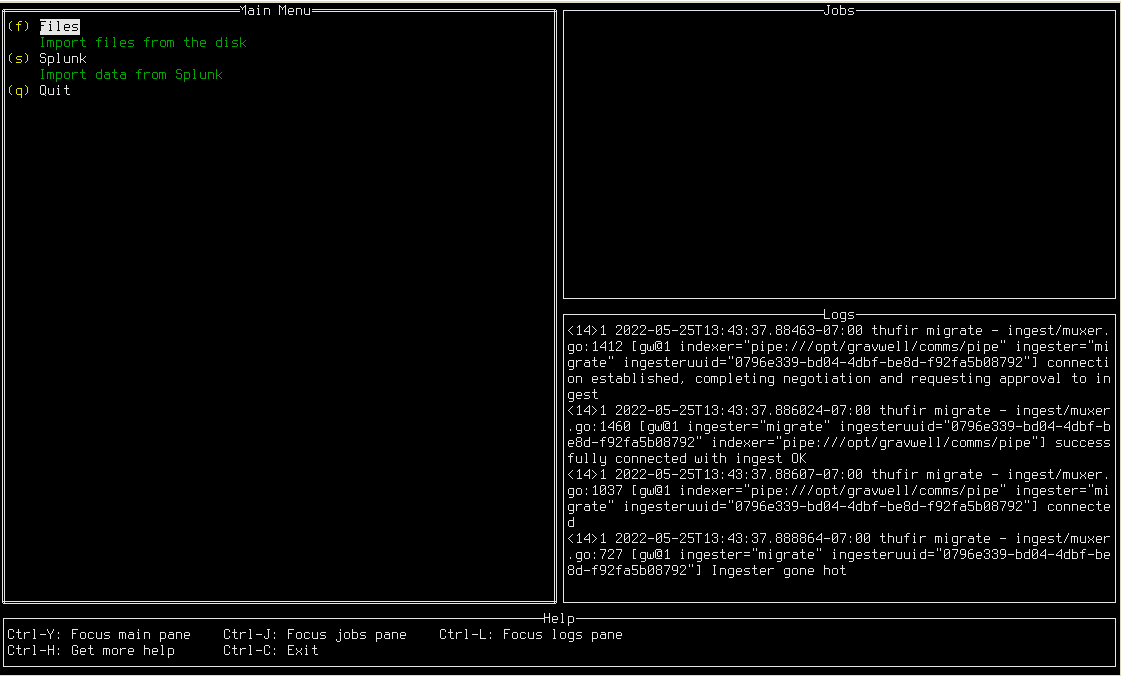
\includegraphics[width=0.95\linewidth]{images/migrate-ui.png}
	\caption{The migration tool UI}
	\label{fig:migrate-ui}
\end{figure}

\subsection{Migrating Files}

Importing files from the disk is quite simple. First, set up the configuration file to point at files on the disk you're interested in ingesting. Then, from the main menu, select the "Files" option. You should see a list of all the \code{Files} config blocks you defined. For instance, given the following configuration block, you should see a menu which resembles the screenshot in Figure \ref{fig:filemenu}.

\begin{verbatim}
[Files "auth"]
	Base-Directory="/tmp/log"
	File-Filter="auth.log,auth.log.[0-9]"
	Tag-Name=auth2
	Ignore-Timestamps=true #do not ignore timestamps
	Recursive=true
\end{verbatim}

\begin{figure}
	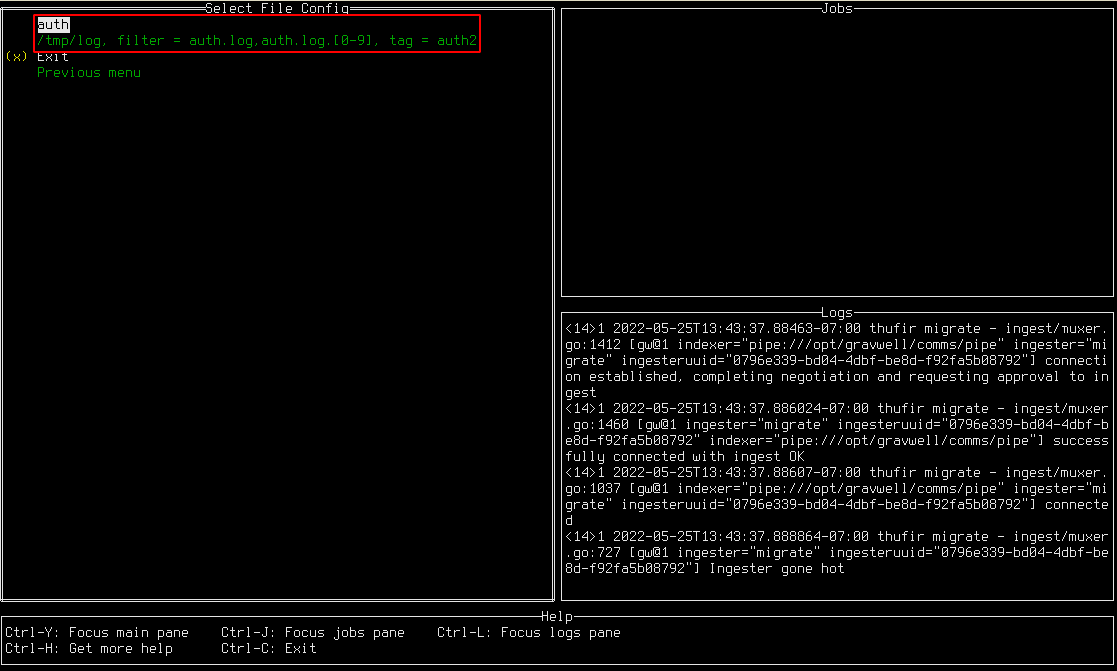
\includegraphics[width=0.95\linewidth]{images/filemenu.png}
	\caption{File migration menu}
	\label{fig:filemenu}
\end{figure}

Selecting ``auth'' opens another menu from which the migration can be launched. To begin the migration, press the `s' key or select the ``Start'' option. As seen in Figure \ref{fig:filejob}, a job will appear in the Jobs pane showing the migration progress. In this case, there were 2 files ingested, for a total of 1444 entries and 141537 bytes of data. 

\begin{figure}
	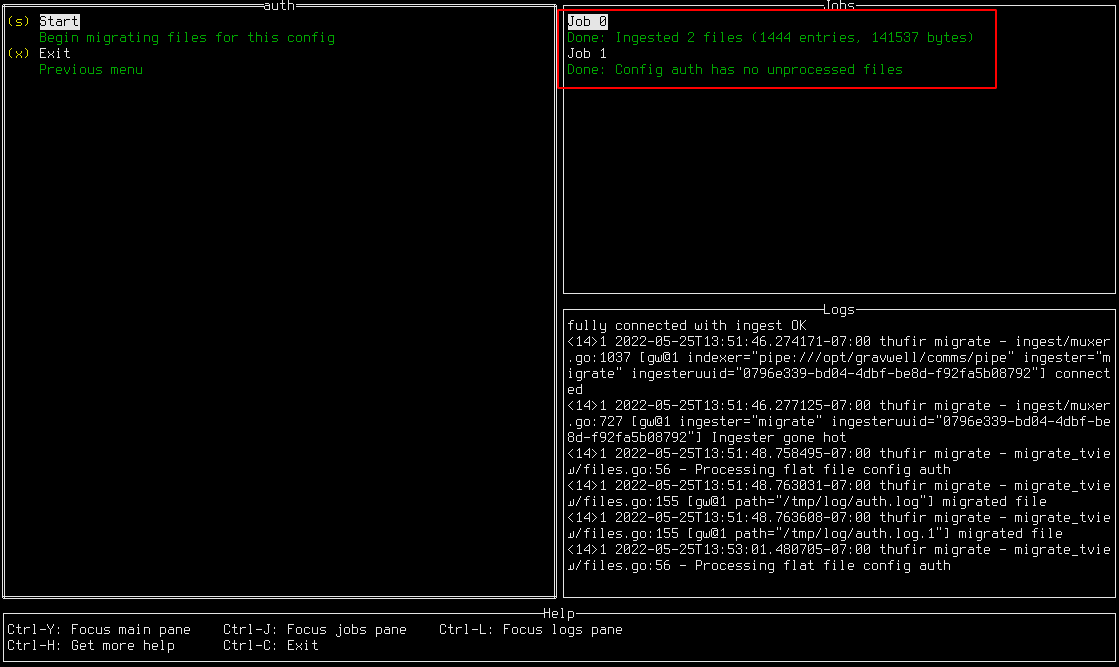
\includegraphics[width=0.95\linewidth]{images/filejob.png}
	\caption{File migration jobs}
	\label{fig:filejob}
\end{figure}

Note that there are actually two jobs shown in the screenshot. After the first migration job completed, ``Start'' was selected again. However, the migration tool tracks how much of each file it has ingested, so it will not duplicate data; the second job simply noted that there was no new data to ingest and exited.

\clearpage
\subsubsection{File Configuration Details}

The migrate tool can have multiple \code{Files} configuration blocks which allows the migrate tool to consume from many different directories, applying tags, custom timestamps, and even custom preprocessors to different batches of files.  If you are performing a very large migration from many different file sources, you can set up a big config file that points at all your sources, fire up the migration jobs, and head home for the weekend.  The `migrate` tool will walk each directory and consume each file according to the given configuration.

A \code{Files} configuration target is defined using the \code{Files} specifier with a unique name. Here is an example looking for files in \code{/tmp/logs}:

\begin{verbatim}
[Files "auth"]
	Base-Directory="/tmp/logs/"
	File-Filter="auth.log,auth.log.[0-9]" #we are looking for all authorization log files
	Tag-Name=auth
\end{verbatim}

The \code{Files} configuration element can contain the parameters in Table \ref{table:files-options}.


\begin{table}
\begin{tabular}{p{0.18\linewidth}p{0.1\linewidth}p{0.35\linewidth}p{0.35\linewidth}}
\textbf{Parameter} & \textbf{Required} & \textbf{Description} & \textbf{Example} \\
\hline
Base-Directory   &   yes      & A full path to the directory containing flat files to be ingested. & \code{Base-Directory=/var/log/auth} \\
File-Filter      &   yes      & A comma separated list of file glob patterns that specify which files to consume. & \code{File-Filter="*.log,file.txt"} \\
Tag-Name         &   yes      & The tag name that the migrate tool should ingest all files into.  This must be a valid tag name. & \code{Tag-Name=auth} \\
Ignore-Timestamps &         & A Boolean value indicating if the migrate tool should not attempt to resolve timestamps, but should instead the timestamp of now. The default value is false. & \code{Ignore-Timestamps=true} \\
Assume-Local-Timezone &     & A Boolean indicating that if the resolved timestamps do not have a timezone, use the local timezone. The default is false, meaning use UTC. & \code{Assume-Local-Timezone=true} \\
Timezone-Override &         & A string indicating that if the resolved timestamps do not have a timezone, use the given timezone. The timezone must be specified in IANA format. & \code{Timezone-Override="America/New\_York"} \\
Recursive &                 & A Boolean indicating that the tool should recurse into any sub-directories found in the \code{Base-Directory} and attempt to match and consume files. Default is false. & \code{Recursive=true} \\
Ignore-Line-Prefix &        & A string which indicates that a line should be ignored.  This can be specified multiple times and is useful for dealing with headers on files. & \code{Ignore-Line-Prefix="\#"} \\
Preprocessor &              & Specify preprocessors to be applied to entries as they are consumed from flat files.  More than one preprocessor can be specified and they are executed in order. & \code{Preprocessor="logins"} \\
\end{tabular}
\caption{Files configuration options}
\label{table:files-options}
\end{table}

Here is an example config snippet which shows the full range of config options for a directory, including the use of a preprocessor:


\begin{verbatim}
[Files "testing"]
	Base-Directory="/tmp/testlogs/"
	File-Filter="app.log,app.log.[0-9],host.log*"
	Tag-Name=apps
	Assume-Local-Timezone=true #Default for assume localtime is false
	Ignore-Timestamps=false
	Recursive=true
	Ignore-Line-Prefix="#"
	Ignore-Line-Prefix="//"
	Preprocessor="loginapps"

[Preprocessor "loginapp"]
	Type=regexextract
	Regex="\\S+ (?P<host>\\S+) \\d+ \\S+ \\S+ (?P<data>\\{.+\\})$"
	Template="{\"host\": \"${host}\", \"data\": ${data}}"
\end{verbatim}

\clearpage

\subsection{Migrating Splunk Data}
\index{Splunk}

The migrate tool can copy data out of a Splunk server and into Gravwell. In Splunk, entries are organized by index and source type; in the migration process, the tool pulls entries out of a given index \& sourcetype and ingests them into a Gravwell tag.

\subsubsection{Configuring Splunk Tokens}

In order to fetch data from a Splunk server, you must generate an authentication token which the migration tool can use to communicate with Splunk. Tokens may be generated in the Splunk UI under Settings > Tokens (Figure \ref{fig:tokensmenu}).

\begin{figure}
	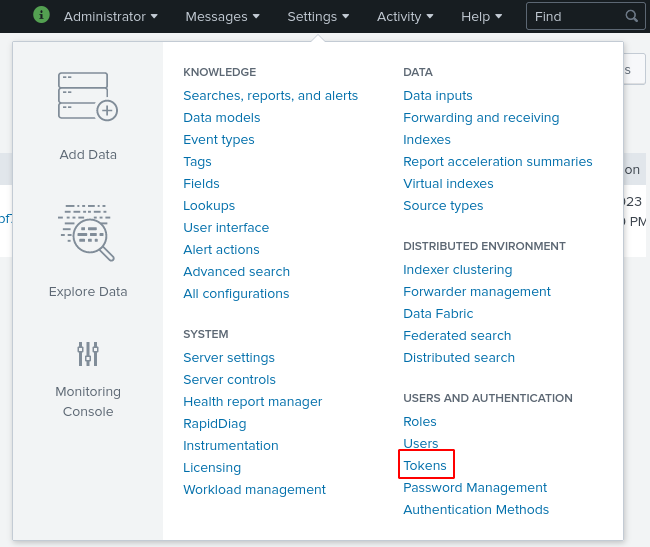
\includegraphics[width=0.8\linewidth]{images/tokensmenu.png}
	\caption{Splunk tokens menu}
	\label{fig:tokensmenu}
\end{figure}

On the Tokens page, click the `New Token' button, then fill in the ``Audience'' field with something like ``Gravwell migration'', select a token expiration time if desired (+60d is a good choice), and click `Create'. The UI will then display a token in the ``Token'' field as seen in Figure \ref{fig:newtoken}; copy this and save it somewhere, because it cannot be retrieved later!

\begin{figure}
	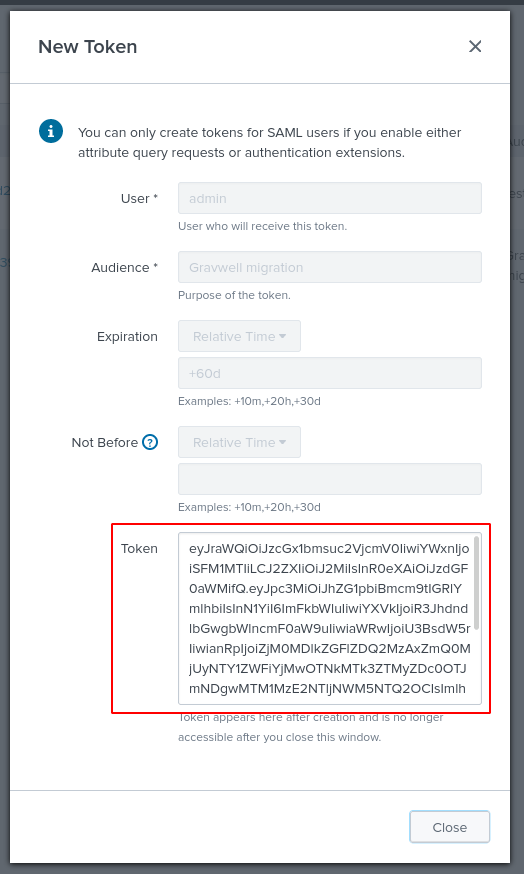
\includegraphics[width=0.8\linewidth]{images/newtoken.png}
	\caption{Newly-generated Splunk token.}
	\label{fig:newtoken}
\end{figure}

This token string should be inserted into the \code{Token} field of a Splunk configuration block in the main config file. The \code{Server} field should correspond to whatever IP address or hostname you use to access your Splunk server.

\clearpage
\subsubsection{Configuring Splunk Migrations}

The migrate tool must know a few basic things about the Splunk server in order to connect:

\begin{itemize}
\item The server's IP or hostname.
\item A valid auth token for the Splunk server.
\end{itemize}

These properties are defined in a \code{Splunk} configuration block within the config file. The simplest version might look like this, defining a server named ``splunk1'':

\begin{verbatim}
[Splunk "splunk1"]
	Token=`eyJraWQiOj[...]nlHnn4Oivew`
	Server=splunk.example.org
\end{verbatim}

Multiple \code{Splunk} blocks may be defined, although each must have a unique name. The parameters shown in Table \ref{table:splunk-config} may be used in a \code{Splunk} config block.


\begin{table}
\begin{tabular}{p{0.18\linewidth}p{0.1\linewidth}p{0.35\linewidth}p{0.35\linewidth}}
\textbf{Parameter} & \textbf{Required} & \textbf{Description} & \textbf{Example} \\
\hline
Server & yes & The hostname or IP address of the Splunk server. Port 8089 must be accessible. & \code{Server=splunk.example.org} \\
Token	 & yes & A valid Splunk auth token. & \code{Token=eyJraWQiOj[...]nlHnn4Oivew} \\
Ingest-From-Unix-Time & & A Unix timestamp which specifies the default ``start'' time to use when copying entries from the Splunk server. This may be overridden on a per-sourcetype basis. & \code{Ingest-From-Unix-Time=1625100000} \\
Index-Sourcetype-To-Tag & & A mapping of a Splunk index and sourcetype pair to a Gravwell tag. Can be set interactively from within the migrate tool. & \code{Index-Sourcetype-To-Tag=main,json:importedjson} (maps the index "main" and sourcetype "json" to the Gravwell tag "importedjson") \\
Preprocessor &              & Specify preprocessors to be applied to entries as they are consumed from Splunk.  More than one preprocessor can be specified and they are executed in order. & \code{Preprocessor="logins"} \\
\end{tabular}
\caption{Splunk config options}
\label{table:splunk-config}
\end{table}

Note: The migrate tool will automatically create a file named \code{splunk1.conf} in \code{/opt/gravwell/etc/migrate.conf.d} to store your index+sourcetype→tag mappings (see below). Settings in this file will be merged with the settings in the main configuration file automatically.

\subsubsection{Importing Splunk Data}

To import data from Splunk, make sure you have configured at least one \code{Splunk} block in the config file (see configuration section above), then select ``Splunk'' from the main menu. This will open a new menu (Figure \ref{fig:splunkserver}) in which you can select which Splunk server to migrate from.

\begin{figure}
	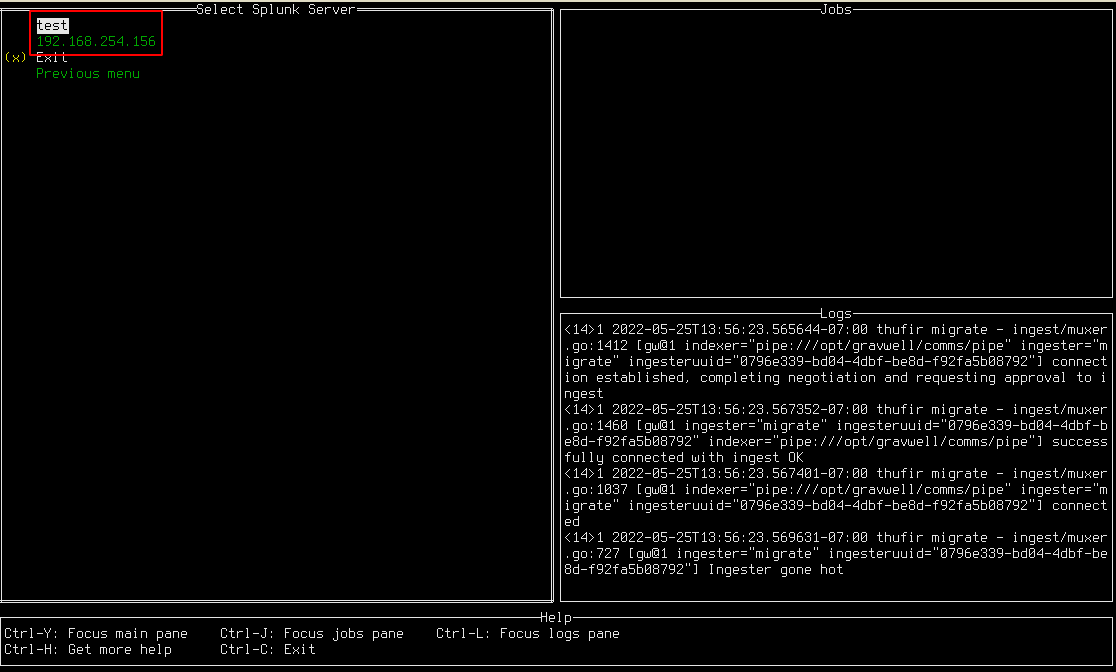
\includegraphics[width=0.95\linewidth]{images/splunkserver.png}
	\caption{Splunk server selection.}
	\label{fig:splunkserver}
\end{figure}

Once a server has been selected, you will see the server's menu (Figure \ref{fig:splunkservermenu})

\begin{figure}
	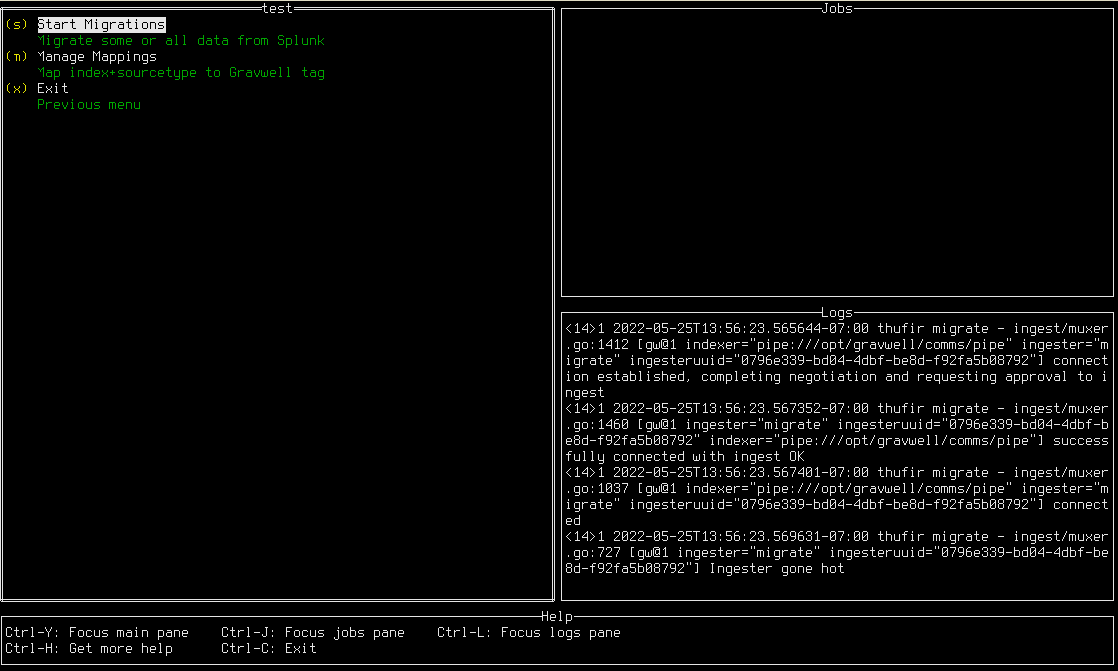
\includegraphics[width=0.95\linewidth]{images/splunkservermenu.png}
	\caption{Splunk server menu.}
	\label{fig:splunkservermenu}
\end{figure}

\clearpage
\subsubsection{Mapping index+sourcetype to tag}

You must now define how Splunk's data organization should be mapped to Gravwell. In Splunk, data is organized into indexes and sourcetypes. In Gravwell, data simply receives a tag. To define these mappings, select ``Manage Mappings''; this will open the mapping screen shown in Figure \ref{fig:splunkmappings}

\begin{figure}
	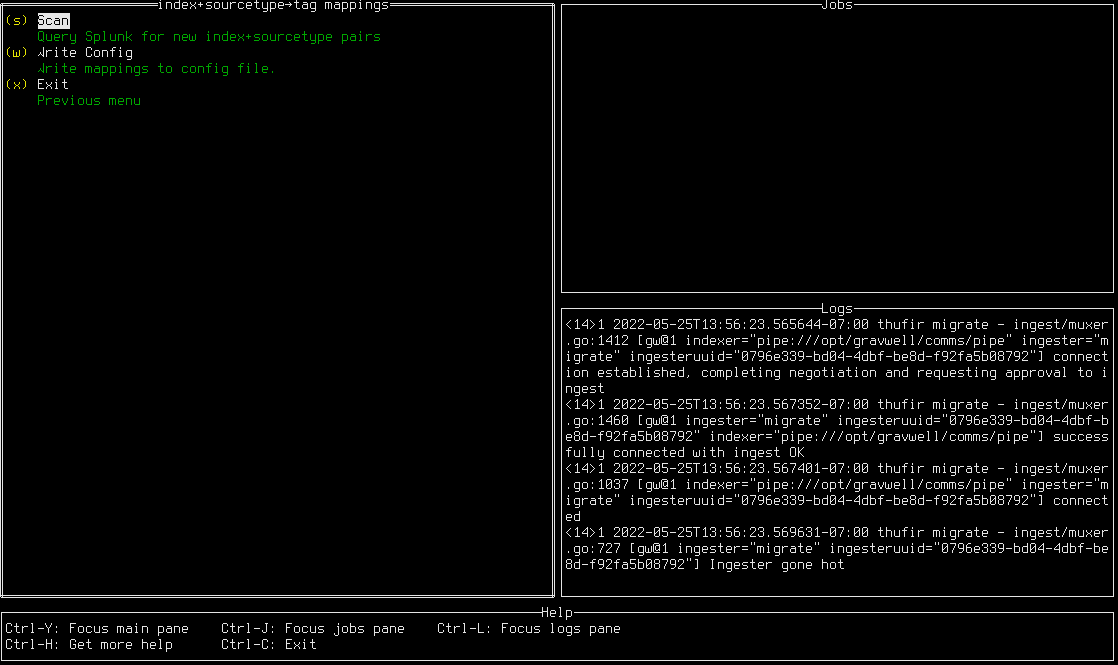
\includegraphics[width=0.95\linewidth]{images/splunkmappings.png}
	\caption{Mapping management menu.}
	\label{fig:splunkmappings}
\end{figure}

Initially, the tool is not aware of which indexes and sourcetypes exist on the Splunk server. Select ``Scan'' to connect to the Splunk server and query this information; this may take a few seconds. Once the scan is complete, several index+sourcetype pairs should be visible, each with a blank tag, as seen in Figure \ref{fig:sourcetypes}.

\begin{figure}
	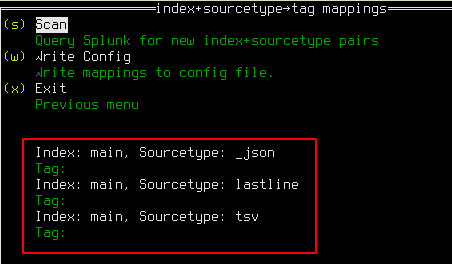
\includegraphics[width=0.95\linewidth]{images/sourcetypes.png}
	\caption{Sourcetype listing.}
	\label{fig:sourcetypes}
\end{figure}

Select a pair which you wish to import and press enter. A form (Figure \ref{fig:tagform}) will be displayed in which you may enter the Gravwell tag to be used; note that it will only allow you to type valid tag characters. You may also set a Unix timestamp to start the migration from, if you wish to exclude old data.

\begin{figure}
	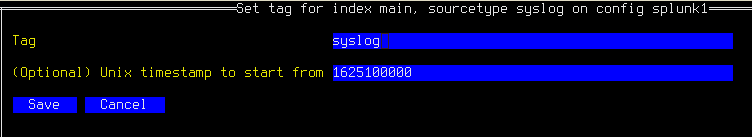
\includegraphics[width=0.8\linewidth]{images/tagform.png}
	\caption{Tag definition form.}
	\label{fig:tagform}
\end{figure}

Note: If the Unix timestamp is set to 0, migration will begin from 1970, which can take a long time to complete even when no data is present. To speed things up, we strongly recommend either setting a timestamp in this form, or setting the \code{Ingest-From-Unix-Time} parameter in the config file (see above).

After you have set the tag for the desired index + sourcetype pairs, you can select ``Write Config'' to write out a file in the \code{migrate.conf.d} directory which will store the mappings permanently.

\subsubsection{Starting Migrations}

Having defined mappings from Splunk index+sourcetype to Gravwell tag, you may now launch migration jobs. From the server menu, select ``Start Migrations''. A menu will appear showing the index+sourcetype → tag mappings you defined earlier. Selecting one of these mappings will start a migration job (Figure \ref{fig:migratejobs}).

\begin{figure}
	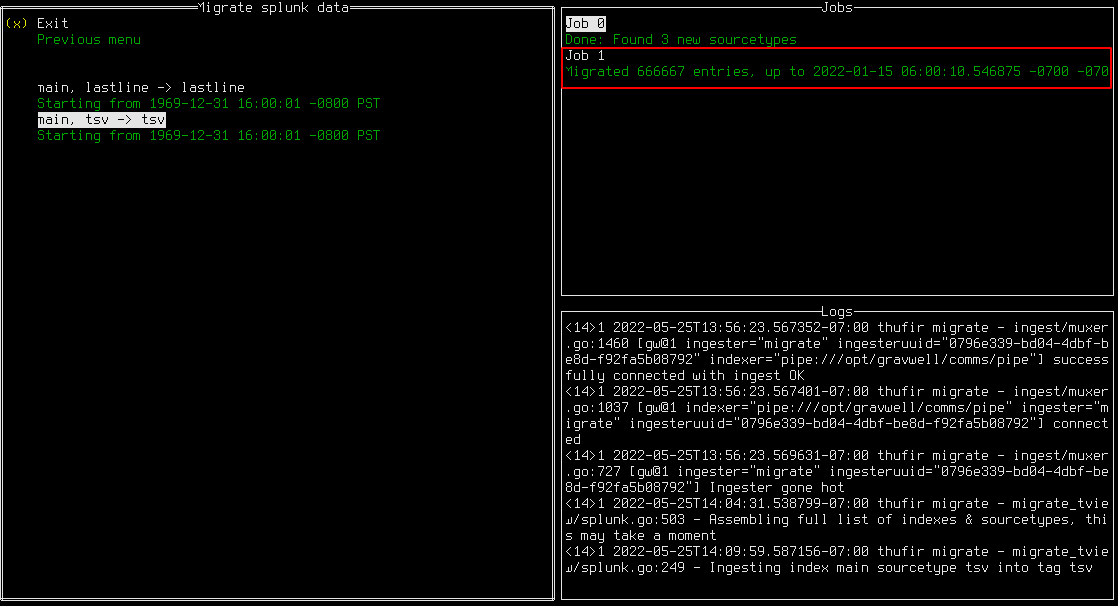
\includegraphics[width=0.95\linewidth]{images/migratejobs.png}
	\caption{Migration jobs.}
	\label{fig:migratejobs}
\end{figure}


You can launch multiple migrations at once. Note that Splunk migrations may take a while; if you exit the migrate tool while a Splunk migration is running, the job will be halted as soon as possible and the most recent timestamp will be stored to resume later--we make every effort to avoid data duplication!

\subsection{Quitting the Tool}

You can exit the migration tool at any time by hitting Ctrl-C, or by backing all the way up to the top-level menu and pressing \code{q}. The tool will gracefully shut down all in-progress migrations and save its state. Note that if a particularly data-heavy Splunk migration job is in progress, it may take several seconds for the data to finish transferring; the UI will notify you that it is still waiting on some jobs and will quit when all are done.



\clearpage

\section{Importing One File}
\index{Ingesters!single file}
The single file ingester is one of the most basic ingesters.  It is designed to ingest a single line-delimited file to a specific tag.  It can transparently decompress files and has some limited parsing ability.  If you have a single large Apache access log or just need to script up some one off file ingestion, it can be the simplest option. The ingester is included in the `gravwell-tools` package for Debian and Redhat, and is also available as a standalone shell installer.. Once installed, the program is located at \code{/usr/local/sbin/gravwell\_single\_file\_ingester}.

The ingester is a standalone ingester that is designed to operate using flags rather than a config file.  This means that it lacks some of the additional functionality of other ingesters such as custom timestamp definitions and preprocessor support.  Pass the \code{-h} flag to the command to get a listing of options:

\begin{verbatim}
  -block-size int
    	Optimized ingest using blocks, 0 disables
  -clean-quotes
    	clean quotes off lines
  -clear-conns string
    	comma seperated server:port list of cleartext targets
  -i string
    	Input file to process (specify - for stdin)
  -ignore-prefix string
    	Ignore lines that start with the prefix
  -ignore-ts
    	Ignore timetamp
  -ingest-secret string
    	Ingest key (default "IngestSecrets")
  -pipe-conn string
    	Path to pipe connection
  -quotable-lines
    	Allow lines to contain quoted newlines
  -source-override string
    	Override source with address, hash, or integeter
  -status
    	Output ingest rate stats as we go
  -tag-name string
    	Tag name for ingested data (default "default")
  -timeout int
    	Connection timeout in seconds (default 1)
  -timestamp-override string
    	Timestamp override
  -timezone-override string
    	Timezone override e.g. America/Chicago
  -tls-conns string
    	comma seperated server:port list of TLS connections
  -tls-private-key string
    	Path to TLS private key
  -tls-public-key string
    	Path to TLS public key
  -tls-remote-verify
    	Validate remote TLS certificates (default true)
  -utc
    	Assume UTC time
  -verbose
    	Print every step
  -version
    	Print version and exit
\end{verbatim}

Most of these flags are optional, but the following are required: At least one indexer must be specified, using \code{-clear-conns}, \code{tls-conns}, \code{pipe-conn}, or a combination thereof. The ingest secret should also be specified with \code{-ingest-secret}, and the desired tag should be specified with \code{-tag}. Finally, the file to ingest must be specified using the \code{-i} flag.

The following command ingests the contents of \code{/tmp/my-logs.txt}, one entry per line. It ignores (does not ingest) any lines starting with the \code{\#} character. It will attempt to extract timestamps from the log entries (the default) but if no timezone is specified in the log entry, it will assume America/Chicago. The entries will be ingested to the indexer at \code{10.0.0.50}.

\begin{verbatim}
/usr/local/sbin/gravwell_single_file_ingester -clear-conns 10.0.0.50 -ingest-secret xyzzy123 -timezone-override "America/Chicago" -ignore-prefix "#" -status -i /tmp/my-logs.txt
\end{verbatim}

\section{Importing PCAP Files}
\index{Ingesters!PCAP file}
If you have existing PCAP files (from Wireshark or tcpdump or some other packet capture tool), you can ingest them using the PCAP file ingester.  The ingester is included in the `gravwell-tools` package for Debian and Redhat, and is also available as a standalone shell installer. After installation, the program is found in \code{/usr/local/sbin/gravwell\_pcap\_file\_ingester}.

The ingester is a standalone ingester that is designed to operate using flags rather than a config file.  This means that it lacks some of the additional functionality of other ingesters such as custom timestamp definitions and preprocessor support.  Pass the \code{-h} flag to the command to get a listing of options:

\begin{verbatim}
  -clear-conns string
    	comma seperated server:port list of cleartext targets
  -ingest-secret string
    	Ingest key (default "IngestSecrets")
  -no-ingest
    	Do not ingest the packets, just read the pcap file
  -pcap-file string
    	Path to the pcap file
  -pipe-conn string
    	Path to pipe connection
  -source-override string
    	Override source with address, hash, or integeter
  -tag-name string
    	Tag name for ingested data (default "default")
  -timeout int
    	Connection timeout in seconds (default 1)
  -tls-conns string
    	comma seperated server:port list of TLS connections
  -tls-private-key string
    	Path to TLS private key
  -tls-public-key string
    	Path to TLS public key
  -tls-remote-verify
    	Validate remote TLS certificates (default true)
  -ts-override
    	Override the timestamps and start them at now
  -version
    	Print the version information and exit
\end{verbatim}

Most of these flags are optional, but the following are required: At least one indexer must be specified, using \code{-clear-conns}, \code{tls-conns}, \code{pipe-conn}, or a combination thereof. The ingest secret should also be specified with \code{-ingest-secret}, and the desired tag should be specified with \code{-tag}. Finally, the ingest file must be specified using the \code{-pcap-file} flag.

The following ingests the packets in \code{/tmp/netflow-capture.pcap} to an indexer on the local machine. Each packet is ingested as a single entry.

\begin{verbatim}
/usr/local/sbin/gravwell_pcap_file_ingester -pipe-conns /opt/gravwell/comms/pipe 
-ingest-secret MyIngestSecret -pcap-file /tmp/netflow-capture.pcap
\end{verbatim}


